\section{Validating RDF}
RDF therefore allows to represent and store data, and with this ability emerges the need to validate that the schema of the graph is correct. In order to perform the validation of RDF data there  have been previous attempts, described in \refsec{ch02-validating-other-techs}, this dissertation will focus on Shape Expressions. But in order to validate RDF data every technology will need to face the following RDF concepts:

\begin{itemize}
 \item the form of a node (the mechanisms for doing this will be called “node constraints”);
 \item the number of possible arcs incoming/outgoing from a node; and
 \item the possible values associated with those arcs.
\end{itemize}

\begin{figure}[hb]
  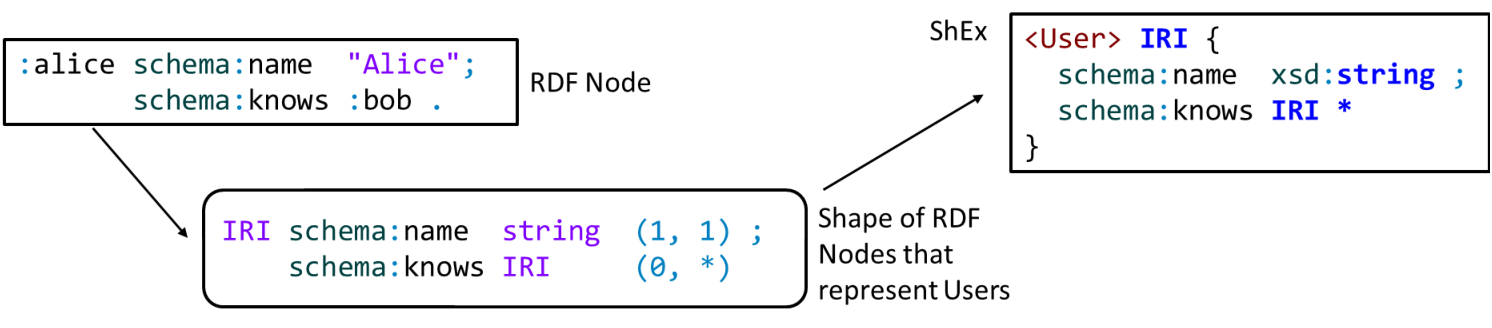
\includegraphics{rdf-node-and-shape}
  \caption[RDF node and its shape]{RDF node and its shape.}
  \labfig{rdf-graph}
\end{figure}

\reffig{rdf-graph} illustrates those RDF concepts by means of the Shape Expression that validates users. There we can see that the shape of the RDF node that represents Users represents the form of a node, the number of possible arcs and the possible value associated with those arcs.

\subsection{Shape Expressions}
As defined in \sidecite{labra-validating-rdf} Shape Expressions (ShEx) is a schema language for describing RDF graphs structures. ShEx was originally developed in late 2013 to provide a human-readable syntax for OSLC Resource Shapes. It added disjunctions, so it was more expressive than Resource Shapes. Tokens in the language were adopted from Turtle and SPARQL with tokens for grouping, repetition and wildcards from regular expression and RelaxNG Compact Syntax \sidecite[-10pt]{van2003relax}. The language was described in a paper \sidecite{eric-rdf-validation-lang} and codified in a June 2014 W3C member submission which included a primer and a semantics specification. This was later deemed “ShEx 1.0”.

As of publication, the ShEx Community Group was starting work on ShEx 2.1 to add features like value comparison and unique keys. See the ShEx Homepage \url{http://shex.io/} for the state of the art in ShEx. A collection of ShEx schemas has also been started at \url{https://github.com/shexSpec/schemas}.

\begin{figure}[hb]
\begin{lstlisting}
PREFIX :       <http://example.org/>
PREFIX schema: <http://schema.org/>
PREFIX xsd:  <http://www.w3.org/2001/XMLSchema#>

:User {
  schema:name          xsd:string  ;
  schema:birthDate     xsd:date?  ;
  schema:gender        [ schema:Male schema:Female ] OR xsd:string ;
  schema:knows         IRI @:User*
}
\end{lstlisting}
\caption[Shape Expression Example]{Shape Expression Example. This example describes a shape expression that describes a user as a node that has one name of type string, an optional bithd date of type date, one gender of type Male, Female or free string and a set between 0 and infinite of other users represented by the knows property.}
\labfig{shape-expr-ex}
\end{figure}

\subsubsection{ShEx Compact Syntax: \texttt{ShExC}}
The ShEx compact syntax (ShExC) was designed to be read and edited by humans. It follows some conventions which are similar to Turtle or SPARQL.

\begin{itemize}
	\item \texttt{PREFIX} and \texttt{BASE} declarations follow the same convention as in Turtle. In the rest of this chapter we will omit prefix declarations for brevity.
	\item Comments start with a \texttt{\#} and continue until the end of line.
	\item The keyword a identifies the \texttt{rdf:type} property.
	\item Relative and absolute IRIs are enclosed by \texttt{< >} and prefixed names (a shorter way to write out IRIs) are written with prefix followed by a colon.
	\item Blank nodes are identified using \texttt{\_:label} notation.
	\item Literals can be enclosed by the same quotation conventions ( \texttt{'}, \texttt{"}, \texttt{'''}, \texttt{"""}) as in Turtle.
	\item Keywords (apart from a) are not case sensitive. Which means that \texttt{MinInclusive} is the same as \texttt{MININCLUSIVE}.
\end{itemize}

A ShExC document declares a ShEx schema. A ShEx schema is a set of labeled shape expressions which are composed of node constraints and shapes. These constrain the permissible values or graph structure around a node in an RDF graph. When we are considering a specific node, we call that node the focus node.

\begin{figure}[hb]
  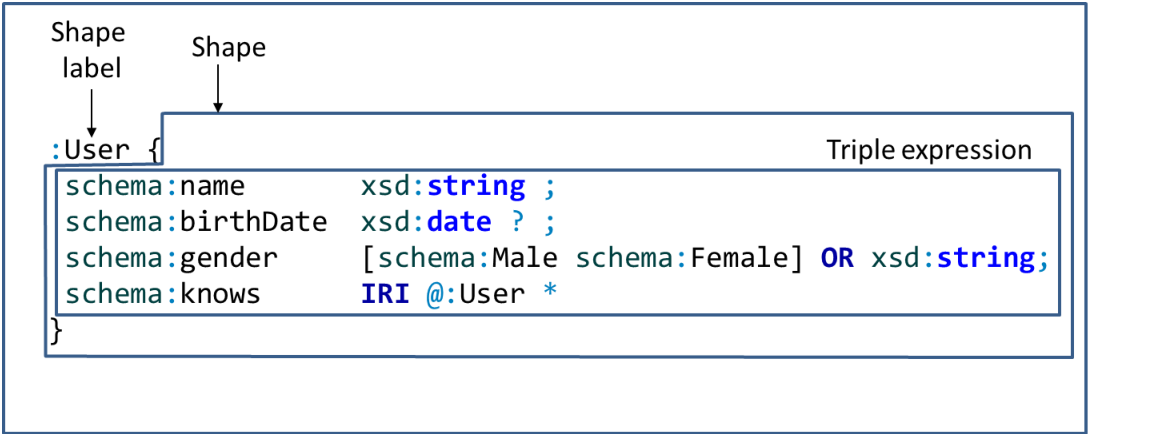
\includegraphics{shex-out}
  \caption[Shapes, shape expression labels and triple expressions]{Shapes, shape expression labels and triple expressions.}
  \labfig{shex-out-view}
\end{figure}

\reffig{shex-out-view} shows the first level of a shape expression, we have a label and the shape itself that is what we asing to the \texttt{:User} label. Then, the shape is composed by triple expressions. The triple expression structure is explained in \reffig{shex-triple-expression}, and as its name indicates it is composed of three elements, the property, the node constraint and the cardinality.

\begin{figure}[hb]
  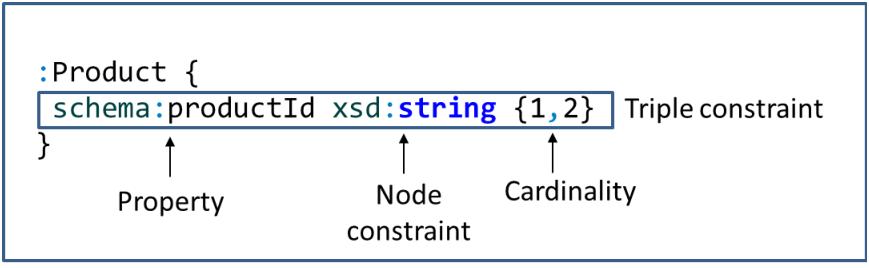
\includegraphics{shex-triple-expression}
  \caption[Parts of a triple expression]{Parts of a triple expression.}
  \labfig{shex-triple-expression}
\end{figure}

Shape Expressions Compact Syntax is much bigger and containts other multiple features that give ShEx its power, and all of them can be explored in \sidecite{labra-validating-rdf} but they are not needed to understand this dissertation.

\subsubsection{Use of ShEx}
Strictly speaking, a ShEx schema defines a set of graphs. This can be used for many purposes, including communicating data structures associated with some process or interface, generating or validating data, or driving user interface generation and navigation. At the core of all of these use cases is the notion of conformance with schema. Even one is using ShEx to create forms, the goal is to accept and present data which is valid with respect to a schema.
ShEx has several serialization formats:

\begin{itemize}
	\item a concise, human-readable compact syntax (ShExC);
	\item a JSON-LD syntax (ShExJ) which serves as an abstract syntax; and
	\item an RDF representation (ShExR) derived from the JSON-LD syntax.
\end{itemize}

These are all isomorphic and most implementations can map from one to another.
Tools that derive schemas by inspection or translate them from other schema languages typically generate ShExJ. Interactions with users, e.g., in specifications are almost always in the compact syntax ShExC. As a practical example, in HL7 FHIR, ShExJ schemas are automatically generated from other formats, and presented to the end user using compact syntax. See Section 6.2.3 for more details.
ShExR allows to use RDF tools to manage schemas, e.g., doing a SPARQL query to find out whether an organization is using dc:creator with a string, a foaf:Person, or even whether an organization is consistent about it.

\subsubsection{ShEx Implementations} \todo{Check links.}
At the time of this writing, we are aware of the following implementations of ShEx.

\begin{itemize}
	\item shex.js for Javascript/N3.js (Eric Prud’hommeaux) \url{https://github.com/shexSpec/shex.js/};
	\item Shaclex for Scala/Jena (Jose Emilio Labra Gayo) \url{https://github.com/labra/shaclex/};
	\item shex.rb for Ruby/RDF.rb (Gregg Kellogg) \url{https://github.com/ruby-rdf/shex};
	\item Java ShEx for Java/Jena (Iovka Boneva/University of Lille) \url{https://gforge.inria.fr/projects/shex-impl/}; and
	\item ShExkell for Haskell (Sergio Iván Franco and Weso Research Group) \url{https://github.com/weso/shexkell}.
\end{itemize}

There are also several online demos and tools that can be used to experiment with ShEx.

\begin{itemize}
	\item shex.js (http://rawgit.com/shexSpec/shex.js/master/doc/shex-simple.html);
	\item Shaclex (http://shaclex.herokuapp.com); and
	\item ShExValidata (for ShEx 1.0) (https://www.w3.org/2015/03/ShExValidata/).
\end{itemize}

\subsection{Other Technologies}\labsec{ch02-validating-other-techs}
As other validation technologies we will just explore the existence of them as it is very interesting to know how other tools approach the same issue.

\subsubsection{SHACL}
Also in \sidecite{labra-validating-rdf}, Chapter 5, it is fully explained that Shapes Constraint Language (SHACL) has been developed by the W3C RDF Data Shapes Working Group, which was chartered in 2014 with the goal to “produce a language for defining structural constraints on RDF graphs \sidecite{oslc-resource-shape}.”
The main difference that made us choose ShEx over SHACL are that ShEx emphasized human readability, with a compact grammar that follows traditional language design principles and a compact syntax evolved from Turtle.

\subsubsection{JSON Schema}
JSON Schema born as a way to validate JSON-LD, and as turtle and RDF can be serialized as JSON-LD it is usual to think that JSON Schema can validate RDF data, but this is not fully correct. And the reason is that the serialization of RDF data in to JSON-LD is not deterministic, that means that a single schema might have multiple serializations, which interferes with the validation as you cannot define a relative schema.
